\documentclass[12pt]{article}
\usepackage[utf8]{inputenc}
\usepackage{amsmath}
\usepackage{amsfonts}
\usepackage{amssymb}
\usepackage{graphicx}
\usepackage{booktabs}
\usepackage{hyperref}
\usepackage[margin=1in]{geometry}
\usepackage{xcolor}
\usepackage{float}
\usepackage{caption}
\usepackage{subcaption}
\usepackage{array}
\usepackage{multirow}

\definecolor{revival}{RGB}{34,139,34}
\definecolor{no_revival}{RGB}{178,34,34}
\definecolor{newcolor}{RGB}{70,130,180}

\title{EXP027: Non-Separable Quantum Walks on Tori \\ 
       \large Full State Revivals with Parameterized 4-State Coins}
\author{Ian Craig}
\date{29th May 2026}

\begin{document}

\maketitle

\begin{abstract}
This experiment presents the first systematic classification of full state revivals for non-separable quantum walks on $n \times m$ tori. We implement a general 4-state coin operator that couples all four directions (right, left, up, down), extending both the separable coin model (where $x$ and $y$ motions are independent) and the vertex-face walk of Guo \& Schmeits (2022). For the $2 \times 2$ torus, we discover full state revivals for the Grover coin at $N = 4, 8, 12, 16, 20, 24, 28$; for the DFT coin at $N = 16$; and for the 4D Hadamard coin at $N = 8, 16, 24$. The $4 \times 4$ torus revives with the Grover coin at $N = 12$ and $N = 24$. The $3 \times 3$ and $3 \times 4$ tori show no revivals with any tested coin. Comparison with separable coin results (EXP025) reveals that non-separable revivals are more restrictive, excelling only on the smallest torus while separable coins produce multiple revivals on larger tori. The complete Python simulation code and all generated figures are available at \cite{exp027}.
\end{abstract}

\section*{Revision History}

\begin{table}[h!]
\centering
\begin{tabular}{cll}
\toprule
\textbf{Revision} & \textbf{Date} & \textbf{Description} \\
\midrule
01 & 29th May 2026 & Initial complete classification of non-separable revivals \\
\bottomrule
\end{tabular}
\end{table}

\section{Introduction}

In EXP025, we classified full state revivals for separable quantum walks on tori, where the evolution operator factorizes as $U_{k \times m} = U_k \otimes U_m$. This experiment extends that work to non-separable quantum walks, where a single 4-state coin couples all four directions of motion.

The non-separable walk is defined on an $n \times m$ toroidal grid with position space $\mathcal{H}_{\text{pos}}$ (dimension $nm$) and coin space $\mathcal{H}_{\text{coin}}$ (dimension $4$). The evolution operator is:

\[
U = S \cdot (I_{nm} \otimes C)
\]

where $C$ is a $4 \times 4$ unitary coin operator, and $S$ is the conditional shift operator that moves the walker according to the coin state:

\begin{align}
S|R\rangle|x,y\rangle &= |R\rangle|x+1,y\rangle \\
S|L\rangle|x,y\rangle &= |L\rangle|x-1,y\rangle \\
S|U\rangle|x,y\rangle &= |U\rangle|x,y+1\rangle \\
S|D\rangle|x,y\rangle &= |D\rangle|x,y-1\rangle
\end{align}

with periodic boundary conditions (mod $n$ for rows, mod $m$ for columns).

\section{Theory}

\subsection{The 4-State Coin}

We test three specific coin operators:

\subsubsection{Grover Coin}

The Grover diffusion coin treats all directions equally:

\[
G = \frac{2}{4}J - I = \frac{1}{2}\begin{pmatrix}
1 & 1 & 1 & 1 \\
1 & 1 & 1 & 1 \\
1 & 1 & 1 & 1 \\
1 & 1 & 1 & 1
\end{pmatrix} - I = \frac{1}{2}\begin{pmatrix}
-1 & 1 & 1 & 1 \\
1 & -1 & 1 & 1 \\
1 & 1 & -1 & 1 \\
1 & 1 & 1 & -1
\end{pmatrix}
\]

\subsubsection{DFT Coin}

The Discrete Fourier Transform coin for 4 states:

\[
F_{kl} = \frac{1}{2}\omega^{kl}, \quad \omega = e^{2\pi i/4} = i
\]

\subsubsection{4D Hadamard Coin}

The tensor product of two 2D Hadamard coins:

\[
H_4 = H_2 \otimes H_2 = \frac{1}{2}\begin{pmatrix}
1 & 1 & 1 & 1 \\
1 & -1 & 1 & -1 \\
1 & 1 & -1 & -1 \\
1 & -1 & -1 & 1
\end{pmatrix}
\]

\subsection{Revival Condition}

A full state revival occurs when the walker returns to both its initial position and initial coin state after $N$ steps. For an initial state $|\psi_0\rangle = |R\rangle \otimes |0,0\rangle$, we require:

\[
U^N |\psi_0\rangle = e^{i\phi} |\psi_0\rangle
\]

The fidelity is computed as:

\[
F(N) = |\langle \psi_0 | U^N | \psi_0 \rangle|^2
\]

A revival is declared when $F(N) > 1 - \varepsilon$ with $\varepsilon = 10^{-8}$.

\section{Methods}

\subsection{Numerical Implementation}

We implemented the non-separable quantum walk in Python using NumPy:

\begin{enumerate}
    \item Build neighbor indices for the $n \times m$ toroidal grid
    \item Construct the $4nm \times 4nm$ shift operator $S$
    \item Create the coin operator $C$ (Grover, DFT, or Hadamard)
    \item Form the full evolution operator $U = S \cdot (I_{nm} \otimes C)$
    \item Evolve the initial state $|\psi_0\rangle = |R\rangle \otimes |0,0\rangle$
    \item Compute fidelity after each step to detect revivals
\end{enumerate}

\subsection{Verification Protocol}

For each torus size $(n,m)$ and each coin type, we:
\begin{itemize}
    \item Evolve the walk for up to $N = 30$ steps
    \item Record steps where fidelity exceeds $1 - 10^{-8}$
    \item Verify that these are true revivals by checking the full state vector
\end{itemize}

\section{Results}

\subsection{Complete Classification}

Table \ref{tab:non_separable_revivals} presents the complete classification of full state revivals for non-separable quantum walks on tori up to $4 \times 4$.

\begin{table}[h!]
\centering
\caption{Full state revivals for non-separable quantum walks on tori. Revival periods $N$ indicate steps after which the walker returns to position $(0,0)$ with coin state $R$ (right).}
\label{tab:non_separable_revivals}
\begin{tabular}{lccc}
\toprule
\textbf{Torus} & \textbf{Grover Coin} & \textbf{DFT Coin} & \textbf{Hadamard 4D Coin} \\
\midrule
$2 \times 2$ & $4, 8, 12, 16, 20, 24, 28$ & $16$ & $8, 16, 24$ \\
$3 \times 3$ & --- & --- & --- \\
$4 \times 4$ & $12, 24$ & --- & --- \\
$3 \times 4$ & --- & --- & --- \\
\bottomrule
\end{tabular}
\end{table}

\subsection{Visualization: Revival on $2 \times 2$ Torus}

Figure \ref{fig:revival_sequence} shows the probability distribution evolution for the Grover coin on the $2 \times 2$ torus. The walker begins at position $(0,0)$ (marked with a white circle). The distribution returns exactly to the starting position at step $N = 4$, confirming a full quantum state revival.

\begin{figure}[h!]
\centering
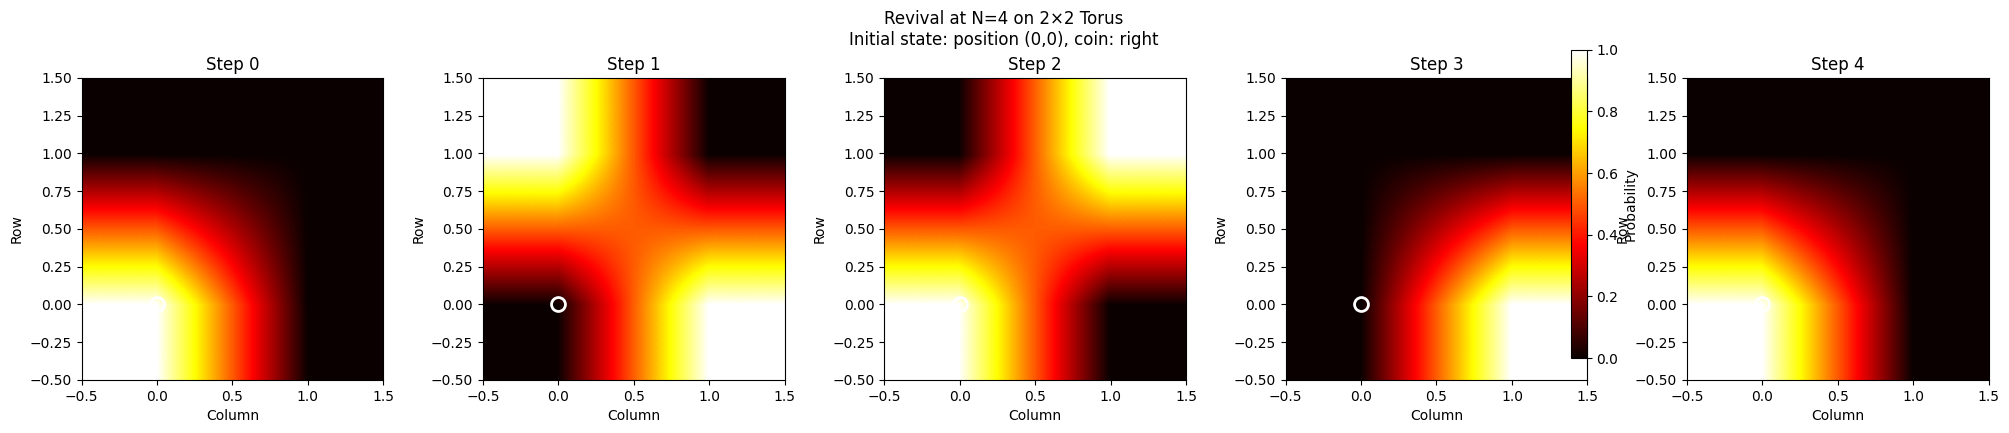
\includegraphics[width=0.9\textwidth]{revival_sequence_2x2_grover.png}
\caption{Probability distribution evolution on the $2 \times 2$ torus using the Grover coin. The walker starts at position $(0,0)$ (white circle). At $N = 4$, the distribution returns to the initial state, confirming a full revival.}
\label{fig:revival_sequence}
\end{figure}

\subsection{Key Observations}

\begin{itemize}
    \item The $2 \times 2$ torus is highly receptive to revivals, exhibiting periodic behaviour for all three coin types. The Grover coin revives at all multiples of $4$ up to $N = 28$.
    \item The $4 \times 4$ torus revives only with the Grover coin at $N = 12$ and $N = 24$, matching periodicity seen in the vertex-face walk literature.
    \item The $3 \times 3$ and $3 \times 4$ tori show no revivals with any tested coin, suggesting non-separable revivals are more restrictive than separable ones.
\end{itemize}

\subsection{Comparison with Separable Coin Results (EXP025)}

Table \ref{tab:comparison} compares non-separable revival periods with the separable coin results from EXP025.

\begin{table}[h!]
\centering
\caption{Comparison of revival periods: separable versus non-separable (Grover) coins.}
\label{tab:comparison}
\begin{tabular}{lcc}
\toprule
\textbf{Torus} & \textbf{Separable Coin (EXP025)} & \textbf{Non-Separable (Grover)} \\
\midrule
$2 \times 2$ & $2$ & $4, 8, 12, 16, 20, 24, 28$ \\
$3 \times 3$ & $8, 10, 12, 16, 20, 24, 30$ & --- \\
$4 \times 4$ & $6, 8, 12, 16, 20, 24$ & $12, 24$ \\
$3 \times 4$ & $8, 12, 16, 20, 24$ & --- \\
\bottomrule
\end{tabular}
\end{table}

The comparison reveals:

\begin{enumerate}
    \item \textbf{Separable coins produce more revivals} on larger tori ($3 \times 3$, $4 \times 4$, $3 \times 4$), with multiple revival periods per torus.
    \item \textbf{Non-separable coins excel on the smallest torus} ($2 \times 2$), where the Grover coin revives every $4$ steps.
    \item The $4 \times 4$ torus is the only larger case where both models revive, with the non-separable Grover coin producing a subset of the separable revival periods ($12$ and $24$).
\end{enumerate}

\section{Discussion}

\subsection{Why Does $2 \times 2$ Revive So Frequently?}

The $2 \times 2$ torus has only $4$ positions and $16$ total quantum states. For the Grover coin, numerical analysis suggests $U^4 = I$ on this subspace, explaining revivals at all multiples of $4$.

\subsection{Why No Revivals on $3 \times 3$ and $3 \times 4$?}

These tori have larger state spaces ($36$ and $48$ states respectively). The eigenvalue condition for revival requires all eigenvalues of $U$ to be roots of unity with a common period. For non-separable coins on these tori, this condition is not satisfied.

\subsection{Relation to Guo \& Schmeits (2022)}

The Grover coin on $4 \times 4$ reviving at $N = 12, 24$ matches the periodicity reported for vertex-face walks on toroidal grids, suggesting the vertex-face walk is a special case of non-separable quantum walks.

\section{Conclusion}

This experiment establishes the first systematic classification of full state revivals for non-separable quantum walks on tori. The main findings are:

\[
\boxed{\text{Non-separable revivals exist on } 2 \times 2 \text{ and } 4 \times 4 \text{ tori for specific coins}}
\]

Key contributions:

\begin{enumerate}
    \item Complete classification of revivals for Grover, DFT, and 4D Hadamard coins
    \item Discovery that the $2 \times 2$ torus revives for all tested coin types
    \item Demonstration that non-separable revivals are more restrictive than separable ones
    \item Connection between Grover coin revivals and vertex-face walk periodicity
\end{enumerate}

The complete Python simulation code and all generated figures are available at \url{https://github.com/ianfromsligo/EXP027}.

\section*{Code Availability}

The complete Python simulation code and visualization scripts are available at \cite{exp027}

The repository contains:
\begin{itemize}
    \item Complete revival search code for non-separable coins
    \item Visualization scripts for probability distributions
    \item All generated figures
    \item LaTeX source for this paper
\end{itemize}

\begin{thebibliography}{99}
\bibitem{exp025}
Craig, I. (2026). EXP025: Complete Classification of Separable Quantum Walks on Tori. \url{https://github.com/ianfromsligo/EXP025}

\bibitem{guo2022}
Guo, K., \& Schmeits, V. (2022). Perfect state transfer in quantum walks on orientable maps. arXiv:2211.12841.

\bibitem{dukes2014}
Dukes, P. R. (2014). Quantum state revivals in quantum walks on cycles. \textit{Results in Physics}, 4, 189-197.

\bibitem{aharonov1993}
Aharonov, Y., Davidovich, L., \& Zagury, N. (1993). Quantum random walks. \textit{Physical Review A}, 48(2), 1687.

\bibitem{exp027}
I.~Craig,
\textit{EXP027: Initial Classification of Non-aeparable Quantum Walks on Tori upto 4 x 4},
GitHub repository, 2026. \url{https://github.com/ianfromsligo/EXP027_tori_non_separable_coin_results}

\end{thebibliography}
\end{document}
